% TeX template for WUEST Call for Applications, gonna be used for other types
% of docs as well, i guess

% written by softbobo - September 2019

% TO DO
% - insert hard facts dummies
% - correct sizing for images in annex
% - find proper font to set


\documentclass[a4paper, 11pt]{article}

\usepackage{fontenc}
\usepackage{multicol}
\usepackage{graphicx}
\usepackage{hyperref}

\begin{document}

%removes page numbers and stuff
\pagestyle{empty}

\section*{The Event}

\section*{Your Role}

% this is double column to save space and be better to read
\section*{Hard Facts}

\begin{multicols}{2}

\textbf{Date:} \\
\textbf{Doors Open:} \\
\textbf{Concerts Between:} \\
\textbf{Address:} \\
\textbf{First Concert:} \\
\href{www.duckduckgo.com}{dummy link} \\
\textbf{Second Concert:} \\
\href{www.duckduckgo.com}{dummy link} \\
\textbf{Contact:} \\

    
\end{multicols}

\section*{WUEST}
WUEST is a team of six individuals with diverse backgrounds in music and club 
culture formed in early 2019. Apart from their individual projects, they 
teamed up to pursue events which are in between music, performance, and 
technology. In the process, they fill unusual spaces with happenings that 
bring new perspectives to known places. This also involves pushing the boundaries 
of well-known event formats. \\
Up until now, the young project cooperated with the independent WUK Theater space 
in Halle, Germany. Examples of this cooperation were the interpretation of the
question for a Better Life as a concert and how society changes through 
technology during the Futur event series. \\
WUEST is responsible for the conceptualization and planning of events together 
with its partners. As a whole, this includes conception, curation, technical 
realisation and artist relations.


\section*{Annex: Pictures}

\begin{figure}
    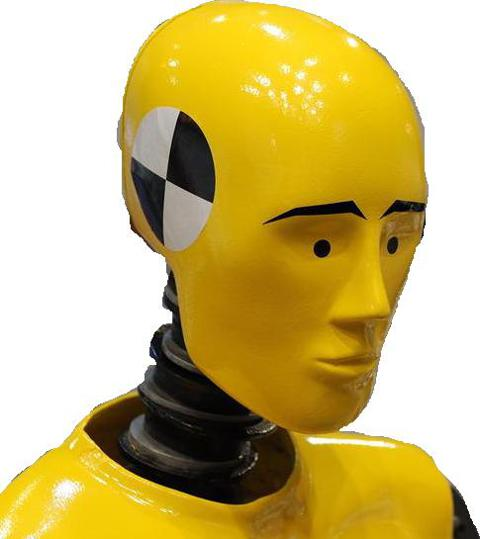
\includegraphics[scale=1.0]{dummy_web_page.jpg}
    \caption{SOURCE: Dummy figure}
\end{figure}

\end{document}